\documentclass[5pt]{article}
\usepackage[letterpaper, margin=1in]{geometry}
\usepackage{graphicx}
\usepackage{booktabs}
\usepackage{subcaption}

\begin{document}

\title{Assignment 4}
\author{Mukul Sati [msati3@gatech.edu]}
\maketitle

I used the CAFFE framework~\cite{jia2014caffe} for my implementation.

\begin{figure*}[T]
  \centering{}
  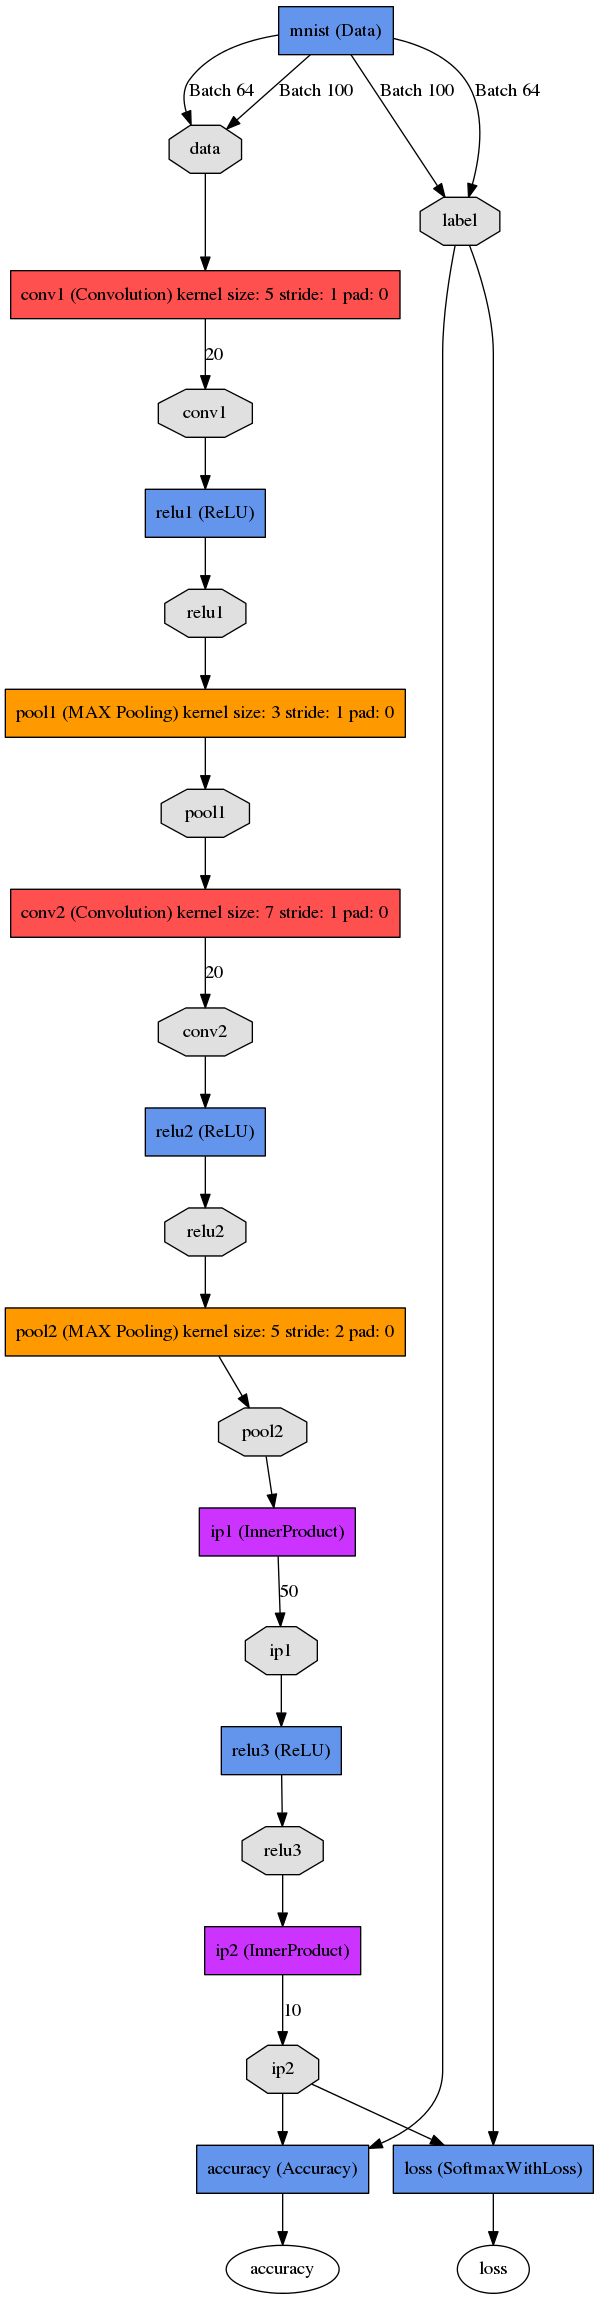
\includegraphics[width=0.35\textwidth]{images/mnist_arch1.png}
  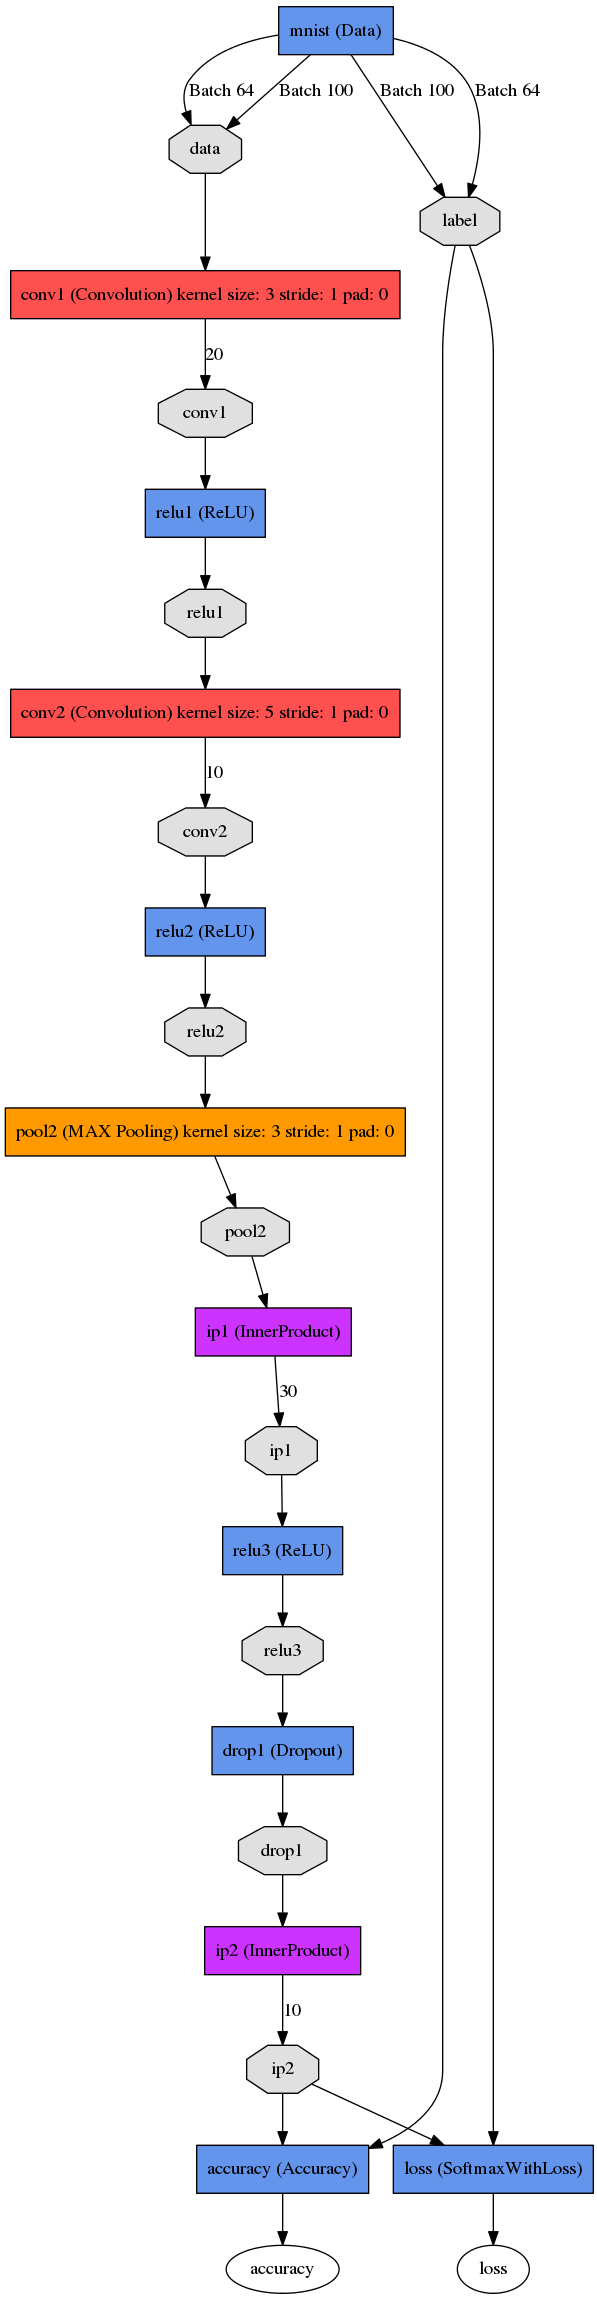
\includegraphics[width=0.35\textwidth]{images/mnist_arch2.png}
  \caption{The two architectures trained for the MNIST dataset.}
\label{fig:mnist_architectures}
\end{figure*}

\section{MNIST Dataset}
I trained two CNN architectures on the MNIST dataset
(Fig.~\ref{fig:mnist_architectures}). For the first architecture, I have a
baseline training loss of 2.41 and a baseline test accuracy of 0.1167 and I
obtain a final accuracy of $99.03\%$. Getting good numbers on the first
architecture, I wanted to simplify the second architecture. Thus, the second
architecture is essentially the first architecture with XXa. For the second
architecture, I have a baseline training loss of $XX$ and a baseline test
accuracy of $XX$ and obtain a final accuracy of $XX$. The training progress is
shown in Fig.~\ref{fig:mnist_learning}.  As I did not manually tweak
hyper-parameters, I feel it was sufficient have directly using the provided
test set during the testing phase instead of performing hold out validation.
The kernels learned from the first and second convolutional layers are
visualized in Fig.~\ref{fig:mnist_kernels}. The confusion matrices of the two
architectures are shown in Fig.~\ref{fig:mnist_confusion}, and a few incorrectly
classified images are shown in Fig.~\ref{fig:mnist_incorrect}.

The following are the gradient descent equations:

\begin{figure}[T]
  \centering{}
  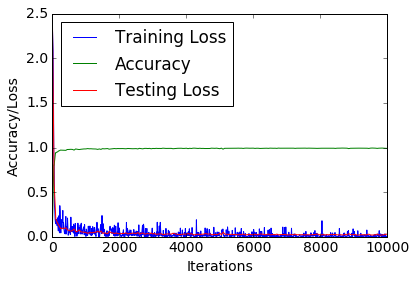
\includegraphics[width=0.4\textwidth]{images/mnist_learning1.png}
  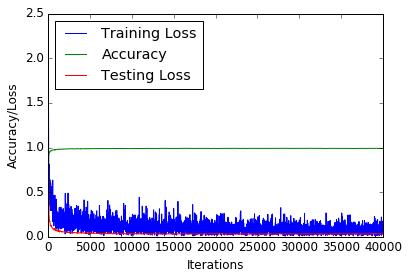
\includegraphics[width=0.4\textwidth]{images/mnist_learning2.png}
  \caption{Training loss and testing loss and accuracy versus iterations for
  architecture 1 (left) and architecture 2 (right).}
\label{fig:mnist_learning}
\end{figure}

\begin{figure}[T]
  \centering{}
  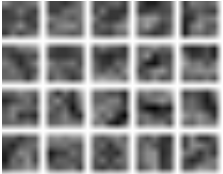
\includegraphics[width=0.35\textwidth]{images/mnist_kernels11.png}
  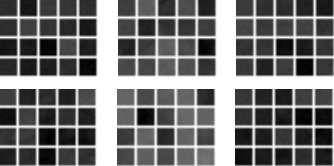
\includegraphics[width=0.5\textwidth]{images/mnist_kernels12.png}
  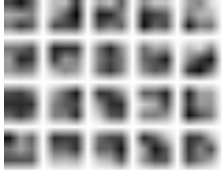
\includegraphics[width=0.3\textwidth]{images/mnist_kernels21.png}
  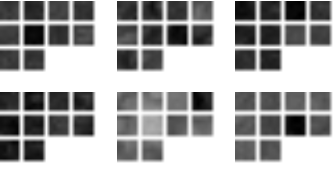
\includegraphics[width=0.5\textwidth]{images/mnist_kernels22.png}
  \caption{The learned filters for the first and some of the learned filters
  for the second convolutional layers of the first (top row) and second
  (bottom row) architectures.}
\label{fig:mnist_kernels}
\end{figure}

\begin{figure}[T]
  \centering{}
  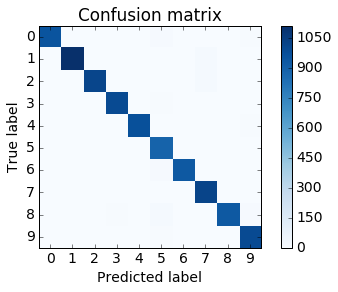
\includegraphics[width=0.4\textwidth]{images/mnist_confusion1.png}
  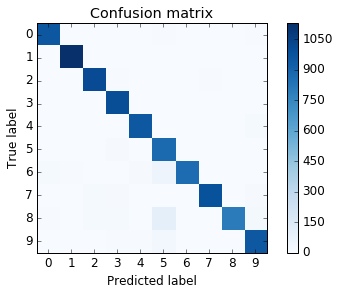
\includegraphics[width=0.4\textwidth]{images/mnist_confusion2.png}
  \caption{Confusion matrix for the first (left) and second (right) 
  architectures.}
\label{fig:mnist_confusion}
\end{figure}

\begin{figure}[T]
  \centering{}
  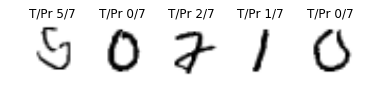
\includegraphics[width=0.4\textwidth]{images/mnist_incorrect1.png}
  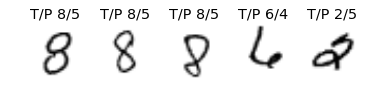
\includegraphics[width=0.4\textwidth]{images/mnist_incorrect2.png}
  \caption{Some incorrectly classified test examples for the first (left)
  and second (right) architectures, showing also the true (T) and predicted
  (Pr) labels.}
\label{fig:mnist_incorrect}
\end{figure}

\section{Sunset Dataset}
I used the CaffeNet pre-trained network that comes with CAFFE\@. This is pretty
similar to AlexNet, but without the relighting data-augmentation and has a
difference in the order of the pooling and normalization layers. The primary
tweaks I made to CaffeNet are:
\begin{enumerate}
  \item Editing the last fully connected layer for the binary classification
    problem at hand. The initial architecture was for the 1000 class ImageNet
    database.
  \item Lowering the learning rate of the solver, while using a higher
    multiplier for the weights of the modified layer.
\end{enumerate}

Using a very small number of training iterations, I quickly arrive to an
accuracy of about $89\%$ (Fig.~\ref{fig:sunset_vanilla_learning}). After a
longer duration of training, the rate stabilizes at $XX\%$

\begin{figure}[h]
  \centering{}
  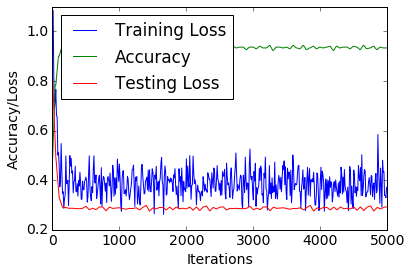
\includegraphics[width=0.8\columnwidth]{images/sunset_vanilla_learning.png}
  \caption{Training loss and testing loss and accuracy versus iterations for
  the vanilla CaffeNet described above.}
\label{fig:sunset_vanilla_learning}
\end{figure}

I use the following schemes for data-augmentation

\medskip
\bibliographystyle{unsrt}
\bibliography{references}

\end{document}
